\documentclass[twocolumn,norwegian]{article}
\usepackage{hyperref}
\hypersetup{colorlinks=true}
\usepackage{titling}
\usepackage{graphicx}

%\setlength{\droptitle}{-1cm} 

%opening
\title{TEK9020 - Prosjektoppgave 1}
\author{Kristoffer Langstad \\ kristoffer.langstad@its.uio.no}
\date{}

\begin{document}

\maketitle

\section{Introduksjon}
I denne oppgaven er tanken å illustrere hva som skjer i mønstergjenkjenning. Ved å bruke tre forskjellige klassifikatorer; Minimum feilrate med normalfordelings antagelse, Minste kvadraters metode og Nærmeste-nabo, skal jeg forsøke å finne ut hvilken av disse tre mønstergjenkjenningsklassifikatorene som er den beste klassifikatoren av tre ulike datasett med forskjellige objekter og egenskaper. Klassifikatorene blir vurdert ved å estimere feilrater med et to-klasse problem. Klassifikatorene trenes opp med et trenings sett og blir evaluert med et test sett for å finne den beste klassifikatoren. Dette gjøres med programmeringsverktøyet Python. Til slutt diskuteres resultatene, og det svares på noen relevante spørsmål angående resultatene som er funnet og om klassifikatorene som er brukt.


\section{Metode}
\subsection{Datasett}
Hvert av de tre datasettene inneholder forskjellige antall objekter og antall egenskaper, som er fordelt på to klasser. Datasett 1 inneholder 300 objekter med 4 egenskaper, datasett 2 inneholder 300 objekter med 3 egenskaper og datasett 3 inneholder 400 objekter med 4 egenskaper. Datasettene blir så individuelt delt inn i 50\% trening og 50\% test datasett, der trenings data består av odde nummererte objekter mens test data består av like nummererte objekter.

\subsection{Trening og evaluering}
Først skal nærmeste-nabo klassifikatoren brukes til å regne ut de beste egenskapskombinasjonene for hver dimensjon for hvert datasett. Her regnes det ut feilrate for hver egenskapskombinasjon, der den egenskapskombinasjonen hver dimensjon som har den laveste feilraten dømmes som den beste egenskapskombinasjonen. 

Når dette er gjort for samtlige egenskapskombinasjoner for et datasett, så skal alle klassifikatorene evalueres. Kun de beste egenskapskombinasjonene hver dimensjon brukes til å bestemme hvilken av de tre klassifikatorene som best klarer å klassifisere objektene i datasettene riktig. Den klassifikatoren med lavest feilrate for den gitte egenskapskombinasjonen anses som den beste klassifikatoren i dette tilfellet. Dette gjøres da for alle tre datasettene.

For å evaluere klassifikatorene benyttes feilrateestimatet som regnes ut som forholdet mellom antall feilklassifiserte objekter og det totale antall objekter i testsettet:
\begin{equation}
	\hat{P}(e) = \frac{n_{feil}}{n_{totalt}}
\end{equation}


\section{Resultater}
\subsection{Finne best egenskapskombinasjonene}
Først finner vi de beste egenskapskombinasjonene med nærmest-nabo klassifikatoren for hver dimensjon for all tre datasettene. Feilrate resultatene av disse vises i Tabell \ref{tab:Dim1} til \ref{tab:Dim4}.
\begin{table}[h!]
	\centering
	%\hskip-2.5cm
	%\rule{0pt}{10pt}
	\begin{tabular}{| c | c  c  c |}
		\hline
		\rule{0pt}{10pt}Dim=1 & Datasett 1 & Datasett 2 & Datasett 3 \\
		\hline
		\rule{0pt}{10pt}1 & \textbf{0.240} & \textbf{0.180} & 0.330 \\
		2 & 0.360 & 0.280 & \textbf{0.310} \\
		3 & 0.4333 & 0.4933 & 0.345 \\
		4 & 0.3867 & - & 0.395 \\
		\hline
	\end{tabular}
	\caption{Feilratene for alle egenskapene i 1 dimensjon, for de tre datasettene. Den beste egenskapen med lavest feilrate for hvert datasett er markert i svart, manglende egenskaper er markert med en strek.}
	\label{tab:Dim1}
\end{table}
\begin{table}[h!]
	\centering
	%\hskip-2.5cm
	%\rule{0pt}{10pt}
	\begin{tabular}{| c | c  c  c |}
		\hline
		\rule{0pt}{10pt}Dim=2 & Datasett 1 & Datasett 2 & Datasett 3 \\
		\hline
		\rule{0pt}{10pt}12 & 0.180 & \textbf{0.0133} & 0.215 \\
		13 & 0.1933 & 0.1933 & 0.170 \\
		14 & \textbf{0.1667} & - & 0.285 \\
		23 & 0.320 & 0.2867 & \textbf{0.095} \\
		24 & 0.2267 & - & 0.240 \\
		34 & 0.300 & - & 0.190 \\
		\hline
	\end{tabular}
	\caption{Feilratene for alle egenskapene i 2 dimensjoner, for de tre datasettene. Den beste egenskapen med lavest feilrate for hvert datasett er markert i svart, manglende egenskaper er markert med en strek.}
	\label{tab:Dim2}
\end{table}
\begin{table}[h!]
	\centering
	%\hskip-2.5cm
	%\rule{0pt}{10pt}
	\begin{tabular}{| c | c  c  c |}
		\hline
		\rule{0pt}{10pt}Dim=3 & Datasett 1 & Datasett 2 & Datasett 3 \\
		\hline
		\rule{0pt}{10pt}123 & 0.1467 & \textbf{0.020} & 0.100 \\
		124 & \textbf{0.100} & - & 0.200 \\
		134 & 0.1267 & - & 0.150 \\
		234 & 0.2133 & - & \textbf{0.075} \\
		\hline
	\end{tabular}
	\caption{Feilratene for alle egenskapene i 3 dimensjoner, for de tre datasettene. Den beste egenskapen med lavest feilrate for hvert datasett er markert i svart, manglende egenskaper er markert med en strek.}
	\label{tab:Dim3}
\end{table}
\begin{table}[h!]
	\centering
	%\hskip-2.5cm
	%\rule{0pt}{10pt}
	\begin{tabular}{| c | c  c  c |}
		\hline
		\rule{0pt}{10pt}Dim=4 & Datasett 1 & Datasett 2 & Datasett 3 \\
		\hline
		\rule{0pt}{10pt}1234 & \textbf{0.0933} & - & \textbf{0.095} \\
		\hline
	\end{tabular}
	\caption{Feilratene for alle egenskapene i 4 dimensjoner, for de tre datasettene. Den beste egenskapen med lavest feilrate for hvert datasett er markert i svart, manglende egenskaper er markert med en strek.}
	\label{tab:Dim4}
\end{table}

\subsection{Evaluere klassifikatorene}
Med de beste egenskapskombinasjonene for hver dimensjon med nærmeste-nabo klassifikatoren, brukes så minimum feilrate og minste kvadraters metode klassifikatorene til å beregne feilrate for å finne ut hvilken av de tre klassifikatorene som gir lavest feilrate og beste resultat for hver egenskapskombinasjon for hvert datasett. Tabellene \ref{tab:Data1}, \ref{tab:Data2} og \ref{tab:Data3} viser henholdsvis resultatene av klassifikator evalueringene for datasett 1, 2 og 3. 

\begin{table}[h!]
	\centering
	%\hskip-2.5cm
	%\rule{0pt}{10pt}
	\begin{tabular}{| c | c  c  c |}
		\hline
		\rule{0pt}{10pt}Beste komb. & N.N. & M.F. & M.K. \\
		\hline
		\rule{0pt}{10pt}1 & 0.240 & \textbf{0.187} & \textbf{0.187} \\
		\hline
		14 & 0.167 & \textbf{0.113} & \textbf{0.113} \\
		\hline
		124 & 0.100 & 0.100 & \textbf{0.0933} \\
		\hline
		1234 & 0.0933 & 0.0800 & \textbf{0.0733} \\
		\hline
	\end{tabular}
	\caption{\textit{Datasett 1}: Feilratene for de beste egenskapskombinasjonene med nærmest-nabo (N.N.), minimum feilrate (M.F.) og minste kvadraters metode (M.K.) klassifikatorene. Den beste klassifikatoren med lavest feilrate for hver egenskapskombinasjon er markert i svart.}
	\label{tab:Data1}
\end{table}
\begin{table}[h!]
	\centering
	%\hskip-2.5cm
	%\rule{0pt}{10pt}
	\begin{tabular}{| c | c  c  c |}
		\hline
		\rule{0pt}{10pt}Beste komb. & N.N. & M.F. & M.K. \\
		\hline
		\rule{0pt}{10pt}1 & 0.180 & \textbf{0.107} & \textbf{0.107} \\
		\hline
		12 & \textbf{0.0133} & 0.020 & 0.120 \\
		\hline
		123 & \textbf{0.020} & \textbf{0.020} & 0.120 \\
		\hline
	\end{tabular}
	\caption{\textit{Datasett 2}: Feilratene for de beste egenskapskombinasjonene med nærmest-nabo (N.N.), minimum feilrate (M.F.) og minste kvadraters metode (M.K.) klassifikatorene. Den beste klassifikatoren med lavest feilrate for hver egenskapskombinasjon er markert i svart.}
	\label{tab:Data2}
\end{table}
\begin{table}[h!]
	\centering
	%\hskip-2.5cm
	%\rule{0pt}{10pt}
	\begin{tabular}{| c | c  c  c |}
		\hline
		\rule{0pt}{10pt}Beste komb. & N.N. & M.F. & M.K. \\
		\hline
		\rule{0pt}{10pt}2 & 0.310 & \textbf{0.225} & 0.335 \\
		\hline
		23 & \textbf{0.095} & 0.200 & 0.200 \\
		\hline
		234 & \textbf{0.075} & 0.130 & 0.160 \\
		\hline
		1234 & 0.095 & \textbf{0.070} & 0.120 \\
		\hline
	\end{tabular}
	\caption{\textit{Datasett 3}: Feilratene for de beste egenskapskombinasjonene med nærmest-nabo (N.N.), minimum feilrate (M.F.) og minste kvadraters metode (M.K.) klassifikatorene. Den beste klassifikatoren med lavest feilrate for hver egenskapskombinasjon er markert i svart.}
	\label{tab:Data3}
\end{table}

\newpage
\subsection{Datasett 2 egenskapsrom visualisert}
I Figur \ref{fig:3DplotDS2} ser vi egenskapsrommet til datasett 2 visualisert i 3 dimensjoner, vinklet for å best mulig vise plasseringene av klasse 1 og 2 objektene utifra egenskapene.

\begin{figure}[ht!]
	\centering
	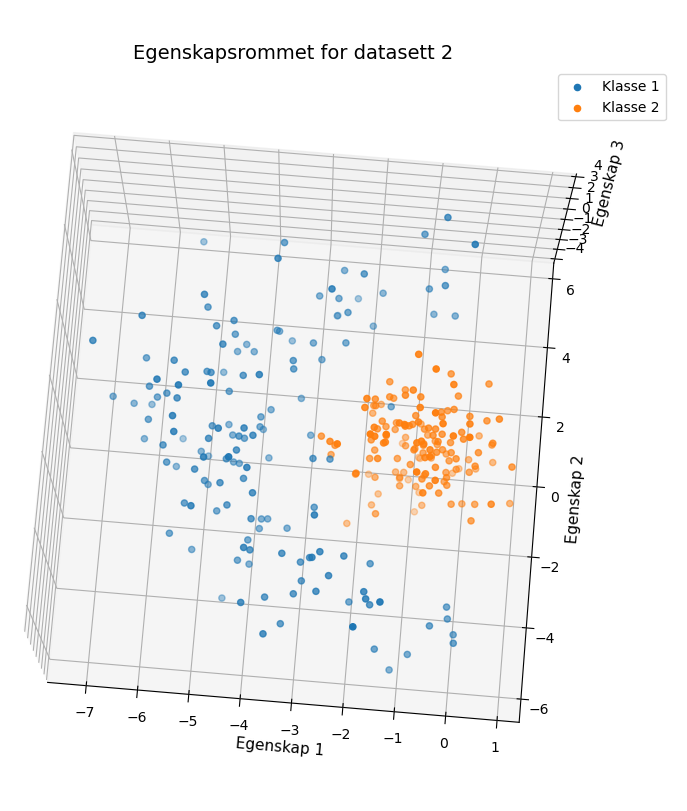
\includegraphics[width=0.9\linewidth]{3DplotDS2.png}
	\caption{Plot av egenskapsrommet til datasett 2 i 3D som viser fordelingen av objekter med klasse 1 (blå) og klasse 2 (oransje). Klasse 2 objektene smaler seg som en klase rundt et punkt, mens klasse 1 objektene ligger i en halvsirkel rundt. \label{fig:3DplotDS2}}
\end{figure}

\section{Diskusjon}
\subsection{Evaluering av nærmeste-nabo klassifikator}
Noe av det som gjør at nærmeste-nabo klassifikatoren egner seg godt til å finne gunstige egenskapskombinasjoner er at den finner egenskaper med dataene som best skiller de forskjellige klassene. Den prøver å finne det punktet i datasettet som er nærmest et annet gitt punkt eller klasse. Den egner seg spesielt godt når det er objekter med flere egenskaper involvert. Den bruker heller ingen antagelser om fordelingen til dataene siden den er en ikke-parametrisk algoritme, som gjør at den fungerer fint på data med ingen eller lite tidligere kunnskap som kan være passende for ikke syntetiske data.

Den har også en relativt rask trenings fase, siden den ikke trenger eksplisitt trening slik at kun treningsegenskapene og tilhørende klassene lagres istedenfor en modell. Når det kommer til test dataene, så må den derimot gå gjennom hele trenings datasettet for å finne det objektet og klassen som er nærmest.

\subsection{Praktisk anvendelse}
Ofte når det kommer til praktiske anvendelser, så kan fort antall dimensjoner på egenskapsrom og størrelsene på trenings dataene blir veldig store. I slike tilfeller kan det fort oppstå feilklassifiseringer siden avstandsberegningene ofte blir mer unøyaktige når dimensjonene øker. Den vil også bruke lang tid under testing, som nevnt allerede, da nærmeste-nabo klassifikatoren må gå gjennom hele trenings settet for å finne kortest avstanden til et objekt for klassifisering. I slike tilfeller kan det da lønne seg å bruke en lineær eller kvadratisk klassifikator. Disse klassifikatorene bruker ofte noe lenger tid på å trenes opp, men har til fordel at de så kan brukes på hele test settet når de først har blitt trent. Dermed holder det å gå gjennom trenings settet kun en gang under treningen, som vil spare tid og minne som trengs.

\subsection{Trening og test data}
Å splitte data inn i trening og test sett er veldig vanlig i mønstergjenkjenning for å trene opp en klassifikator. Dersom test settet skulle vært en del av trenings settet, oppstår det veldig fort overtrening som er lite gunstig for en klassifikator. Når en klassifikator er overtrent på et datasett, så vil det gi veldig bra resultater på det test settet som var en del av treningen men vil den ikke klare å klassifisere et nytt datasett like bra. Med godt trente klassifikatorer vil vi at skal kunne gjøre det bra på generelle datasett og ikke kun på de dataene klassifikatoren har blitt trent opp på. 

\subsection{Rangering av klassifikatorer}
\subsubsection{Datasett 1}
Fra Tabell \ref{tab:Data1} er det enkelt å se at minste kvadraters metode er den beste klassifikatoren på datasett 1. Den er enten like god som minimum feilrate i små dimensjoner eller bedre enn begge de to andre. Siden minste kvadraters metode er en lineær klassifikator, så kan vi konkludere med at datasett 1 som er et syntetisk datasett med trekninger fra kjente tetthetsfordelinger er lineært separabelt. Feilraten minker for alle klassifikatorene når antall egenskaper øker, men minste kvadraters metode har den laveste feilraten og er best på datasett 1 med 4 egenskaper.

\subsubsection{Datasett 2}
Som for datasett 1, er minimum feilrate og minste kvadraters metode klassifikatorene like gode på datasett 2 i en dimensjon. Begge disse to gir dårligere feilrate når dimensjonen øker, mens nærmeste-nabo gir bedre resultater og er best på datasett 2 med 2 egenskaper. Dette kan forklares ved å se på Figur \ref{fig:3DplotDS2}. Der ser vi at de to klassene i datasettet ikke er lineært separable i høyere dimensjoner, og kan ikke bli optimalt separert med en rett linje. Dette passer bedre for f.eks. en kvadratisk klassifikator, som vi kan se i tabellen for datasett 2.

\subsubsection{Datasett 3}
For datasett 3 i Tabell \ref{tab:Data3} er nærmeste-nabo best for dimensjon 2 og 3, mens minimum feilrate er best i dimensjon 1 og 4. Den laveste feilraten på datasett 3 oppnås ved å bruke minimum feilrate klassifikatoren i 4 dimensjoner som er det komplette datasettet med alle 4 egenskapene til objektene.

\section{Konklusjon}
Med nærmeste-nabo klassifikatoren har jeg funnet de beste egenskapskombinasjonene for tre datasett med forskjellig antall objekter og antall egenskaper. Klassifikatorene ble trent med et trenings datasett og evaluert med et test datasett. Med de beste egenskapskombinasjonene har jeg evaluert nærmeste-nabo, minimum feilrate og minste kvadraters metode klassifikatorene for å finne ut hvilken klassifikator som egner seg best på de tre datasettene.

På datasett 1 gav den lineære klassifikatoren minste kvadraters metode den laveste feilraten for alle dimensjoner, med lavest feilrate i 4 dimensjoner. På datasett 2 og 3 gir minste kvadraters metode de dårligste resultatene, mens de to andre ble bedre. På datasett 2 ble den laveste feilraten oppnådd med nærmeste-nabo klassifikatoren med 2 dimensjoner. På datasett 3 ble den laveste feilraten oppnådd med minimum feilrate klassifikatoren med 4 dimensjoner.

\appendix
\section{Python kode}
Koden som er brukt i dette prosjektet kan bli funnet i GitHub på: \url{https://github.com/krilangs/TEK9020/tree/main/Project1}

\end{document}
